\documentclass[a4paper,14pt]{article} % тип документа
%\documentclass[14pt]{extreport}
\usepackage{extsizes} % Возможность сделать 14-й шрифт


\usepackage{geometry} % Простой способ задавать поля
\geometry{top=25mm}
\geometry{bottom=35mm}
\geometry{left=20mm}
\geometry{right=20mm}

\setcounter{section}{0}

%%%Библиотеки
%\usepackage[warn]{mathtext}
%\usepackage[T2A]{fontenc} % кодировка
\usepackage[utf8]{inputenc} % кодировка исходного текста
\usepackage[english,russian]{babel} % локализация и переносы
\usepackage{caption}
\usepackage{listings}
\usepackage{amsmath,amsfonts,amssymb,amsthm,mathtools}
\usepackage{wasysym}
\usepackage{graphicx}%Вставка картинок правильная
\usepackage{float}%"Плавающие" картинки
\usepackage{wrapfig}%Обтекание фигур (таблиц, картинок и прочего)
\usepackage{fancyhdr} %загрузим пакет
\usepackage{lscape}
\usepackage{xcolor}
%\usepackage{indentfirst}
\usepackage[normalem]{ulem}
\usepackage{hyperref}




%%% DRAGON STUFF
\usepackage{scalerel}
\usepackage{mathtools}

\DeclareMathOperator*{\myint}{\ThisStyle{\rotatebox{25}{$\SavedStyle\!\int\!\!\!$}}}

\DeclareMathOperator*{\myoint}{\ThisStyle{\rotatebox{25}{$\SavedStyle\!\oint\!\!\!$}}}

\usepackage{scalerel}
\usepackage{graphicx}
%%% END 

%%%Конец библиотек




%%%Настройка ссылок
\hypersetup
{
colorlinks=true,
linkcolor=blue,
filecolor=magenta,
urlcolor=blue
}
%%%Конец настройки ссылок


%%%Настройка колонтитулы
	\pagestyle{fancy}
	\fancyhead{}
	\fancyhead[L]{Вопрос по выбору}
	\fancyhead[R]{Талашкевич Даниил, группа Б01-009}
	\fancyfoot[C]{\thepage}
%%%конец настройки колонтитулы



\begin{document}
%%%%Начало документа%%%%


%%%Начало титульника
\begin{titlepage}

	\newpage
	\begin{center}
		\normalsize Московский физико-технический институт \\(госудраственный 			университет)
	\end{center}

	\vspace{6em}

	\begin{center}
		\Large Устный экзамен по физике (термодинамика)\\Вопрос по выбору
	\end{center}

	\vspace{1em}

	\begin{center}
		\large \textbf{Термодинамическая устойчивость}
	\end{center}

	\vspace{2em}

	\begin{center}
		\large Талашкевич Даниил\\
		Группа Б01-009
	\end{center}

	\vspace{\fill}

	\begin{center}
	Долгопрудный \\2021
	\end{center}
	
\end{titlepage}
%%%Конец Титульника



%%%Настройка оглавления и нумерации страниц
\thispagestyle{empty}
\newpage
\tableofcontents
\newpage
\setcounter{page}{1}
%%%Настройка оглавления и нумерации страниц


%%%%%%Начало работы с текстом%%%%%%

\section{Алгебра логики}

\subsection{Задача 1}

Согласно условию задачи,
\[ \neg{(x=y)} \land((y<x) \to (2z>x)) \land((x<y) \to (x>2z)) =1\]
Так как это выражение - истина, тогда истине равны:

$a)$ $\neg{(x=y)}=1$ 

$b)$ $(y<x) \to (2z>x)=1$

$c)$ $(x<y) \to (x>2z)=1$ \\

Из пункта а) следует, что $x \neq y$, то есть $x \neq 16$.

Пункт б) выполняется всегда, кроме случая:

\[\begin{cases}
  (y < x) = 1\\
  (2z>x)=0
\end{cases}\] 
\[\begin{cases}
  x>y\\
  x\geqslant 2z
\end{cases}\]
 \[\begin{cases}
  x>16\\
  x\geqslant 14
\end{cases}\]
\[ x>16\]
То есть пункт б) выполняется, если
\[ x\leqslant15\]
Пункт в) отличается от б) только знаками неравенств:
\[ x\geqslant15\]
В итоге получили систему уравнений:
\[\begin{cases}
  x\geqslant15\\
  x\leqslant15\\
  x \neq 16
\end{cases}\]
\[x = 15\]
\begin{flushright}
\begin{large}
\textbf {Ответ: 15}
\end{large}
\end{flushright}

\newpage

\begin{center}
\subsection{Задача 2}
\end{center}
\[f(x,y,z)=\neg{((x \wedge \neg y)\wedge z)}\]
Найдём все значения функции для построения таблицы истинности:
\[f(0,0,0)=\neg{((0 \wedge \neg 0)\wedge 0)}=\neg{(0\wedge 0)}=1\]
\[f(0,0,1)=\neg{((0 \wedge \neg 0)\wedge 1)}=\neg{(0\wedge 1)}=1\]
\[f(0,1,0)=\neg{((0 \wedge \neg 1)\wedge 0)}=\neg{(0\wedge 0)}=1\]
\[f(0,1,1)=\neg{((0 \wedge \neg 1)\wedge 1)}=\neg{(0\wedge 1)}=1\]
\[f(1,0,0)=\neg{((1 \wedge \neg 0)\wedge 0)}=\neg{(1\wedge 0)}=1\]
\[f(1,0,1)=\neg{((1 \wedge \neg 0)\wedge 1)}=\neg{(1\wedge 1)}=0\]
\[f(1,1,0)=\neg{((1 \wedge \neg 1)\wedge 0)}=\neg{(0\wedge 0)}=1\]
\[f(1,1,1)=\neg{((1 \wedge \neg 1)\wedge 1)}=\neg{(1\wedge 0)}=1\]
\begin{center}
\begin{tabular}{|c|c|c|c|}
\hline
$x$ & $y$ & $z$ & $f(x,y,z)$ \\
\hline
0 & 0 & 0 & 1 \\
\hline
0 & 0 & 1 & 1 \\
\hline
0 & 1 & 0 & 1 \\
\hline
0 & 1 & 1 & 1 \\
\hline
1 & 0 & 0 & 1 \\
\hline
1 & 0 & 1 & 0 \\
\hline
1 & 1 & 0 & 1 \\
\hline
1 & 1 & 1 & 1 \\
\hline
\end{tabular}
\end{center}

\newpage
\begin{center}
\subsection{Задача 3}
\end{center}
\[1\oplus x_1 \oplus x_2 = (x_1\rightarrow x_2) \wedge (x_2\rightarrow x_1) \]
Для доказательства рассмотрим, когда (в каких случаях) оба выражения равны истине:\\

$1)$ $f_1(x_1, x_2)= (1\oplus x_1) \oplus x_2 =1$

$ a)$ если $x_1=0,$ то $x_2=0,$

$ b)$ если $x_1=1,$ то $x_2=1,$
То есть $x_1 = x_2,$ если $f_1(x_1, x_2)=1$ \\

$2)$ $f_2(x_1, x_2)= (x_1\rightarrow x_2) \wedge (x_2\rightarrow x_1)=1$

Заметим, что $x_1 = x_2 =0$ или $x_1 = x_2 =1$, иначе возникает ситуация $1\rightarrow 0 = 0$, то есть $x_1 = x_2,$ если $f_2(x_1, x_2)=1$ \\

Оба выражения равны истине только тогда, когда $x_1 = x_2$, в остальных случаях $(x_1 \neq x_2)$ они равны нулю (лжи), то есть булевы функции $f_1(x_1, x_2)$ и $f_2(x_1, x_2)$ ведут себя одинаково при различных $x_1$ и $x_2$, значит они эквивалентны.


\begin{flushright}
\begin{large}
\textbf {Доказано}
\end{large}
\end{flushright}

\begin{center}
\subsection{Задача 4}
\end{center}


$a)$ $x\wedge (y\rightarrow z) =(x\wedge y)\rightarrow(x\wedge z)$\\

Пусть $x=0$, тогда выражение слева в $a)$ всегда равно нулю \[(0\wedge (y\rightarrow z))=0\]

Значит \[(x\wedge y)\rightarrow(x\wedge z)=0\]

\[\begin{cases}
  x\wedge y = 1\\
  x\wedge z = 0
\end{cases}\]
\[x=y=1\]
Получили, что $x=1$, предполагая, что $x=0$.
 \underline{Противоречие. Дистрибутивность не выполянется.}\\
 $b)$ $x\oplus (y \leftrightarrow z) = (x\oplus y)\leftrightarrow (x\oplus z)$ \\

Предположим, что выражение слева $(x\oplus (y \leftrightarrow z))$ равно истине, тогда:
\begin{equation}x\oplus (y \leftrightarrow z)=1
\end{equation}
\begin{equation}(x\oplus y)\leftrightarrow (x\oplus z)=1
\end{equation}

Рассмотрим решение уравнения $(1)$: случай 1:
\[\begin{cases}
  x\oplus y = 1\\
  x\oplus z = 1
\end{cases}\]
\[y=z\neq x\]
Рассмотрим случай 2:
\[\begin{cases}
  x\oplus y = 0\\
  x\oplus z = 0
\end{cases}\]
\[y=z = x\]
В любом случае в решении $(x\oplus y)\leftrightarrow (x\oplus z)=1$ выполняется $y=z$.
  
Решением уравнения $(2)$ являются 2 системы:
 \begin{equation}\begin{cases}
  x = 0\\
  y =z
\end{cases} \end{equation}
 \begin{equation}\begin{cases}
  x = 1\\
  y \neq z
\end{cases} \end{equation}
 То есть одно из решений содержит $y \neq z$, но в решении уравнения $(1)$ всегда $y=z$.
\underline{Противоречие. Дистрибутивность не выполянется.}
\newpage
\begin{center}
\subsection{Задача 5}
\end{center}

$a)$ \underline{Коммутативность для импликации} $x\rightarrow y =y\rightarrow x$ \underline{не выполняется}, так как если $x=0, y=1$, то $0\rightarrow 1=1$, но $1\rightarrow 0=0$ \\

$b)$ \underline{Ассоциативность} $(x\rightarrow y)\rightarrow z = x\rightarrow (y\rightarrow z) $ \underline{не выполняется}, так как при если $x=0$, то $x\rightarrow (y\rightarrow z)=1$ при любых $y$ и $z$, при этом $x\rightarrow y=1$, но если $z=0$, то $(x\rightarrow y)\rightarrow z =0$, в то время как $x\rightarrow (y\rightarrow z)=1$ \\

\subsection{Задача 6}

$a)$ $f(x_1,x_2,x_3)=00111100$

Для наглядности составим  таблицу истинности:
\begin{center}
\begin{tabular}{|c|c|c|c|}
\hline
$x_1$ & $x_2$ & $x_3$ & $f(x_1,x_2,x_3)$ \\
\hline
0 & 0 & 0 & 0 \\
\hline
0 & 0 & 1 & 0 \\
\hline
0 & 1 & 0 & 1 \\
\hline
0 & 1 & 1 & 1 \\
\hline
1 & 0 & 0 & 1 \\
\hline
1 & 0 & 1 & 1 \\
\hline
1 & 1 & 0 & 0 \\
\hline
1 & 1 & 1 & 0 \\
\hline
\end{tabular}
\end{center}

Заметим, что при $x_1=x_2$ выходит $f(x_1,x_2,x_3)=0$, а в других случаях $f(x_1,x_2,x_3)=1$, значит \underline{$x_1$ и $x_2$ - существенные переменные, а $x_3$ - фиктивная.} \\

$b)$ $g(x_1,x_2,x_3)=(x_1\rightarrow (x_1\vee x_2))\rightarrow x_3$

Если $x_1=1$, то $(x_1\rightarrow (x_1\vee x_2))=(1\rightarrow 1)=1$.

Если $x_1=0$, то $(x_1\rightarrow (x_1\vee x_2))=(0\rightarrow (0\vee x_2))=1$.

Получили, что $(x_1\rightarrow (x_1\vee x_2))=1$ не зависит от $x_1$ и тем более от $x_2$, значит $g(x_1,x_2,x_3)=1\rightarrow x_3$.
Итак, \underline{$x_1$ и $x_2$ - фиктивные переменные, а $x_3$ - существенная переменная.}

\newpage
\begin{center}
\subsection{Задача 7}
\end{center}
\[f(x_1,...,x_n)=(x_1\vee f(0,x_2,...,x_n))\wedge (\neg x_1 \vee f(1,x_2,...,x_n))\]

$1)$ Пусть $f(0,x_2,...,x_n)=0$, тогда:
\[f(0,x_2,...,x_n)=(0\vee f(0,x_2,...,x_n))\wedge (1 \vee f(1,x_2,...,x_n))=0\wedge 1 =0\]
Выражение выполняется.

$2)$ Пусть $f(0,x_2,...,x_n)=1$, тогда:
\[f(0,x_2,...,x_n)=(0\vee f(0,x_2,...,x_n))\wedge (1 \vee f(1,x_2,...,x_n))=1\wedge 1 =1\]
Выражение выполняется.

$3)$ Пусть $f(1,x_2,...,x_n)=0$, тогда:
\[f(1,x_2,...,x_n)=(1\vee f(0,x_2,...,x_n))\wedge (0 \vee f(1,x_2,...,x_n))=1\wedge 0 =0\]
Выражение выполняется.

$4)$ Пусть $f(1,x_2,...,x_n)=1$, тогда:
\[f(0,x_2,...,x_n)=(1\vee f(0,x_2,...,x_n))\wedge (0 \vee f(1,x_2,...,x_n))=1\wedge 1 =1\]

Выражение выполняется.

Итак, исходное равенство выполняется для любых функций с любыми значениями $x_1$. Интересно также отметить, что равенство выполняется для любого аргумента $x_i$ $(0\leqslant i\leqslant n)$, так как аргументы являются независимыми.

\newpage
\begin{center}
\subsection{Задача 8}
\end{center}
\[x_1^{\alpha_1}\wedge x_2^{\alpha_2} \wedge ... \wedge x_n^{\alpha_n}=1\]

Равенство возможно только в одном случае: $x_i^{\alpha_i}=1$ $(1\leqslant i\leqslant n)$. Значение $x_i^{\alpha_i}$ зависит от $x_i$ и $\alpha_i$: если $x_i=0$, то $\alpha_i=0$, чтобы $x_i^{\alpha_i}=1$ и если $x_i=1$, то $\alpha_i=1$, чтобы $x_i^{\alpha_i}=1$. Определённому значению $x_i$ соответсвует определённое $\alpha_i$, значит если выбран определённый набор $x_1,...,x_n$, ему будет соответствовать единственный набор $\alpha_1,...,\alpha_n$ \\\\
\begin{flushright}
\begin{large}
\textbf {Доказано}
\end{large}
\end{flushright}

\begin{center}
\subsection{Задача 9}
\end{center}
\[\bigvee \limits_{i, j} (x_i\oplus x_j)=(x_1\vee x_2 \vee ... \vee x_n)\wedge (\overline{x_1} \vee \overline{x_2} \vee ... \vee \overline{x_n}) \]
$1)$ $\bigvee \limits_{i, j} (x_i\oplus x_j)=1$, если хотя бы одна комбинация $x_i$ и $x_j$ отличается по значениям. В этом же случае $(x_1\vee x_2 \vee ... \vee x_n)=1$, так как среди $x_i$ будет по крайней мере одна единица, и $(\overline{x_1} \vee \overline{x_2} \vee ... \vee \overline{x_n})= 1$, так как по крайней мере найдётся одно значение $x_i=0$, а значит $\overline{x_i}=1$. Значит
\[\bigvee \limits_{i, j} (x_i\oplus x_j)=(x_1\vee x_2 \vee ... \vee x_n)\wedge (\overline{x_1} \vee \overline{x_2} \vee ... \vee \overline{x_n})=1 \]

Получается, что равенство в условии выполняется.\\
$2)$ $\bigvee \limits_{i, j} (x_i\oplus x_j)=0$, если все значения $x_i$ равны (0 или 1), значит либо $(x_1\vee x_2 \vee ... \vee x_n)=0$, либо $(\overline{x_1} \vee \overline{x_2} \vee ... \vee \overline{x_n})= 0$, тогда
\[\bigvee \limits_{i, j} (x_i\oplus x_j)=(x_1\vee x_2 \vee ... \vee x_n)\wedge (\overline{x_1} \vee \overline{x_2} \vee ... \vee \overline{x_n})=0 \]

Равенство в условии снова выполняется, значит оно справедливо для любых значений $x_i$.

\newpage
\begin{center}
\subsection{Задача 10}
\end{center}
\par
Пусть булева функция выражается только через связки $\vee$ и $\wedge$. Заметим, что эти связки могут только либо сохранять предыдущие значения выражений (переменных), либо увеличивать их до 1, значит функции, использующие только эти связки - нестрого возрастающие. Получается, что нестрого или строго убывающую функцию эти связки описать не могут (перевести 1 в 0), для этого как минимум требуется использовать связку $\neg$.
Значит существует убывающая функция, которая не может быть описана только связками $\vee$ и $\wedge$.

\section{Множества и логика}

\subsection{Задача 1}

 Верно ли, что для любых множеств A и B выполняется равенство:

\[(A\setminus B)\cap ((A\cup B)\setminus (A\cap B)) = A\setminus B\  ? \]
\begin{center}
\bfseries
{\Large Решение: }
\end{center}


\[(A\setminus B)\cap ((A\cup B)\setminus (A\cap B))= A\setminus B\]

Обозначим $X=A\setminus B$, пусть $x\in X$, тогда $x\in A\cap \overline{B}$, значит можно переписать равенство в условии так:
\[(A\cap \overline{B})\cap ((A\cup B)\cap \overline{(A\cap B)})= A\cap \overline{B}\]

$A\cup B$ - объединение множеств, а $A\cap B$ - пересечение, тогда понятно, что множество $(A\cup B)\cap \overline{(A\cap B)}$ можно заменить на $A\bigtriangleup B$, тогда условие переписывается в виде:
\[(A\cap \overline{B})\cap (A\bigtriangleup B)= A\cap \overline{B}\]

По определению операции "симметричное или"
\[A\bigtriangleup B = (A\cap \overline{B})\cup (B\cap \overline{A})\]

Значит $(A\cap \overline{B})\subseteq (A\bigtriangleup B)$ и справедливо
\[(A\cap \overline{B})\cap (A\bigtriangleup B)= A\cap \overline{B}\]

Это выражение эквивалентно исходному, значит и исходное равенство верно.

\begin{flushright}
\begin{large}
\textbf {Ответ: верно}
\end{large}
\end{flushright}

\newpage
\begin{center}
\subsection{Задача 2}
\end{center}

Верно ли, что для любых множеств A, B и C выполняется равенство: $((A \setminus B) \cup (A \setminus C)) \cap (A \setminus (B \cup C)) = A \setminus (B \cup C) $ ?

\begin{center}
\bfseries
{\Large Решение: }
\end{center}

\[((A\setminus B) \cup (A\setminus C)) \cap (A\setminus(B\cap C))=A\setminus (B\cup C)\]

Для удобства перепишем равенство, пользуясь тем, что $A\setminus B = A\cap \overline{B}$:
\[((A\cap \overline{B}) \cup (A\cap \overline{C})) \cap (A\cap \overline{(B\cap C)})=A \cap \overline{(B\cup C)}\]

Воспользуемся формулой дистрибутивности и законом де Моргана:
\[(A\cap \overline{B}) \cup (A\cap \overline{C})= A\cap (\overline{B} \cup \overline{C}) = A\cap \overline{(B \cap C)}\]

Равенство в условии принимает вид:
\[(A\cap \overline{(B \cap C)})\cap (A\cap \overline{(B\cap C)})=A \cap \overline{(B\cup C)}\]

Очевидно, что
\[(A\cap \overline{(B \cap C)})\cap (A\cap \overline{(B\cap C)}) = (A\cap \overline{(B\cap C)})\]

Тогда равенство принимает вид:
\[A\cap \overline{(B\cap C)} = A \cap \overline{(B\cup C)}\]
\[A\cap (\overline{B} \cup \overline{C}) = A \cap (\overline{B} \cap \overline{C})\]


Понятно, что это равенство неверно.

\begin{flushright}
\begin{large}
\textbf {Ответ: неверно}
\end{large}
\end{flushright}

\newpage
\begin{center}
\subsection{Задача 3}
\end{center}

Верно ли, что для любых множеств A, B и C выполняется равенство: $(A \cap B) \setminus C = (A \setminus C) \cap (B \setminus C)?$
\begin{center}
\bfseries
{\Large Решение: }
\end{center}


\[(A\cap B)\setminus C = (A\setminus C) \cap (B\setminus C)\]

Преобразуем равенство так же, как и в первых двух задача:
\[(A\cap B)\cap \overline{C} = (A\cap \overline{C}) \cap (B\cap \overline{C})\]


В записанном равенстве используются только операции пересечения $\cap$, а они ассоциативны:
\[A\cap B\cap \overline{C} = A\cap \overline{C} \cap B\cap \overline{C} \]
\[A\cap B\cap \overline{C} = A\cap \overline{C} \cap B \]
\[A\cap B\cap \overline{C} = A\cap B \cap \overline{C} \]

Получили верное равенство, значит равенство в условии верно.

\begin{flushright}
\begin{large}
\textbf {Ответ: верно}
\end{large}
\end{flushright}

\newpage
\begin{center}
\subsection{Задача 4}
\end{center}

Верно ли, что для любых множеств A и B выполняется включение $(A \cup B) \setminus (A \setminus B) \subseteq B$?
\begin{center}
\bfseries
{\Large Решение: }
\end{center}


\[(A \cup B) \setminus (A \setminus B) \subseteq B\]

Для анализа этого включения немного его преобразуем:
\[(A \cup B) \cap \overline{(A \cap \overline{B})} \subseteq B\]
\[\overline{(A \cap \overline{B})} \cap (A \cup B)  \subseteq B\]

Очевидно, что $(A \cap \overline{B}) \subseteq A$ и $(A \cap \overline{B}) \cap B =0$. Значит $B\subseteq\overline{(A \cap \overline{B})}$, при этом $\overline{(A \cap \overline{B})} \cap A = B \cap A$ и $\overline{(A \cap \overline{B})} \cap B = B $. Применим дистрибутивность:
\[\overline{(A \cap \overline{B})} \cap (A \cup B)  \subseteq B\]
\[(\overline{(A \cap \overline{B})} \cap A) \cup (\overline{(A \cap \overline{B})} \cap B)  \subseteq B\]

Теперь подставим записанные ранее выражения:
\[(B \cap A) \cup B  \subseteq B\]

Очевидно, что $B\subseteq B$ и $(B \cap A)\subseteq B$, тогда верно и
\[(B \cap A) \cup B  \subseteq B\]

Это включение было получено из включения в условии, значит и включение в условии верно.
\begin{flushright}
\begin{large}
\textbf {Ответ: верно}
\end{large}
\end{flushright}

\newpage
\begin{center}
\subsection{Задача 5}
\end{center}

Пусть P = [10, 40]; Q = [20, 30]; известно, что отрезок A удовлетворяет соотношению

\[((x \in A) \rightarrow (x \in P)) \wedge ((x \in Q) \rightarrow (x \in A)).\]
\begin{center}
\bfseries
{\Large Решение: }
\end{center}

\[((x\in A) \rightarrow (x\in P)) \wedge ((x\in Q) \rightarrow (x\in A))=1\]

Из равенства следует, что:

 \[\begin{cases}
  (x\in A) \rightarrow (x\in P) = 1\\
  (x\in Q) \rightarrow (x\in A) = 1
\end{cases}\]
Первое равенство выполняется всегда, кроме случая:
 \[\begin{cases}
  (x\in A) = 1\\
  (x\in P) = 0
\end{cases}\]
 \[\begin{cases}
  x\in A\\
  x \notin [10,40]
\end{cases}\]
Отсюда получаем:
\[A\subseteq [10,40] \]
Второе равенство выполняется всегда, кроме случая:
\[\begin{cases}
  (x\in Q) = 1\\
  (x\in A) = 0
\end{cases}\]
 \[\begin{cases}
  x\in [20,30]\\
  x \notin A
\end{cases}\]
Отсюда получаем, что $A\subseteq [\alpha,\beta]$, где $\alpha \leqslant 20$, а $\beta \geqslant 30$
Запишем два полученных условия:
 \[\begin{cases}
  A\subseteq [\alpha,\beta]$, где $\alpha \leqslant 20$, а $\beta \geqslant 30\\
  A\subseteq [10,40]
\end{cases}\]
Значит $A\subseteq [\alpha,\beta]$, где $\alpha \in [10,20]$, а $\beta \in [30,40]$
Минимально возможный отрезок $A$ равен 10, максимальный - 30.
\begin{flushright}
\begin{large}
\textbf {Ответ: 1) 30, 2) 10}
\end{large}
\end{flushright}


\newpage
\begin{center}
\subsection{Задача 6}
\end{center}

Про множества A, B, X, Y известно, что $A \cap X = B \cap X, A \cup Y = B \cup Y .$ Верно ли, что тогда выполняется равенство $A \cup (Y \setminus X) = B \cup (Y \setminus X)$?
\begin{center}
\bfseries
{\Large Решение: }
\end{center}


По условию $A\cap X = B\cap X, A\cup Y = B\cup Y$. Предположим, что справедливо
\[A \cup (Y \setminus X) = B \cup (Y \setminus X)\]

Преобразуем равенство следующим образом:
\[A \cup (Y \cap \overline{X}) = B \cup (Y \cap \overline{X})\]
\[(A \cup Y) \cap (A \cup \overline{X}) = (B \cup Y) \cap (B \cup \overline{X})\]

По условию, как уже было записано, $A\cup Y = B\cup Y$, значит
\[(A \cup Y) \cap (A \cup \overline{X}) = (A \cup Y) \cap (B \cup \overline{X})\]

Возьмём дополнение обоих частей равенства, используя закон де Моргана:
\[\overline{(A \cup Y)} \cup (X \cap \overline{A}) = \overline{(A \cup Y)} \cup (X \cap \overline{B})\]

Сделаем маленькое преобразование:
\[(X \cap \overline{A}) = (X \cap \overline{A})\cup \varnothing = (X \cap \overline{A})\cup (X \cap \overline{X}) = X \cap (\overline{A} \cup \overline{X}) = X \cap \overline{(A \cap X)} = X\setminus (A \cap X)\]

Тогда
\[\overline{(A \cup Y)} \cup (X\setminus (A \cap X)) = \overline{(A \cup Y)} \cup (X\setminus (B \cap X))\]

По условию $A\cap X = B\cap X$, значит равенство выполняется.

\begin{flushright}
\begin{large}
\textbf {Ответ: верно}
\end{large}
\end{flushright}

\newpage
\begin{center}
\subsection{Задача 7}
\end{center}
Пусть $A_{1} \supseteq A_{2} \supseteq A_{3} \supseteq \ldots \supseteq A_{n} \supseteq \ldots $ — невозрастающая последовательность множеств.
Известно, что $A_{1} \setminus A_{4} = A_{6} \setminus A_{9}$. Докажите, что $A_{2} \setminus A_{7} = A_{3} \setminus A_{8}$.

\begin{center}
\bfseries
{\Large Решение: }
\end{center}


\[A_1\supseteq A_2 \supseteq A_3 \supseteq ... \supseteq A_n \supseteq ...\]
\[A_1 \setminus A_4 = A_6 \setminus A_9\]

Очевидно, что $A_6 \setminus A_9 \subseteq A_6$, но тогда и $A_1 \setminus A_4 \subseteq A_6$, также по условию $A_6 \subseteq A_4$. Получается, что $A_1 \setminus A_4 \subseteq A_6 \subseteq A_4$, то есть $A_1 \setminus A_4  \subseteq A_4$, но по определению разности множеств $A_1 \setminus A_4  \nsubseteq A_4$ в общем случае. Противоречия не возникает только если $A_1 = A_4$, тогда $A_1 \setminus A_4 = \varnothing \subseteq A_4$.

Описанная выше ситуация возможна только при $A_1 = A_2 = A_3 =  A_4$, а так как по условию $A_1 \setminus A_4 = A_6 \setminus A_9 = \varnothing$, то $A_6 = A_7 = A_8 = A_9$.

Тогда получается, что $A_2 = A_3$ и $A_7 = A_8$ и $A_2 \setminus A_7 = A_3 \setminus A_8$. \\


\begin{flushright}
\begin{large}
\textbf {Доказано}
\end{large}
\end{flushright}


\newpage
\begin{center}
\subsection{Задача 8}
\end{center}

Пусть A, B, C, D — такие отрезки прямой, что $A \bigtriangleup B = C \bigtriangleup D$ (симметрические разности равны). Верно ли, что выполняется включение $A \cap B \subseteq C$?
\newpage
\begin{center}
\bfseries
{\Large Решение: }
\end{center}


\[A\bigtriangleup B = C\bigtriangleup D\]

Пусть $A = (\alpha_0, \alpha_1),B = (\beta_0, \beta_1) $, причём $\alpha_0 < \beta_0 < \beta_1 < \alpha_1 $, то есть $B\subseteq A$. Тогда $A \bigtriangleup B = A \setminus B = (\alpha_0, \beta_0)\cup (\beta_1, \alpha_1)$.

Выберем такие $C$ и $D$, что $C =(\alpha_0, \beta_0), D = (\beta_1, \alpha_1)$ и $C \bigtriangleup D =(\alpha_0, \beta_0)\cup (\beta_1, \alpha_1) $. Тогда получим, что $A \bigtriangleup B = C \bigtriangleup D$, что и написано в условии.

Но тогда $A\cap B = B = (\beta_0, \beta_1) $, а $C = (\alpha_0, \beta_0) $, то есть $(A\cap B)\cap C = \varnothing$, тогда тем более $(A\cap B)\subseteq C $.

\begin{flushright}
\begin{large}
\textbf {Не верно}
\end{large}
\end{flushright}

\begin{center}
\subsection{Задача 9}
\end{center}

 Характеристической функцией множества А называется функция:

\[ X_{A}: U \rightarrow \{0,1\} .\]\\
такая, что

\[ X_{A}(x) = \begin{cases}
1 , x\in A,\\
0 , x\notin A.\\ 
\end{cases}\]\\
Докажите, что

а)$\chi_{A\cap B}(x) = \chi_{A}(x) \cdot \chi_{B}(x);$

б)$\chi_{A\setminus B}(x) = \chi_{A}(x) - \chi_{A}(x) \cdot \chi_{B}(x);$

в)$\chi_{A\cup B}(x) = \chi_A(x) + \chi_{B}(x) - \chi_{A}(x)\cdot \chi_{B} (x);$

г)$\chi_{\overline{A}}(x) = 1 - \chi_{A}(x).$


\begin{center}
\bfseries
{\Large Решение: }
\end{center}


Основываясь на том,что функции алгебры логик аналогичны с теоретико-множественными операторами, получим:\\
a) $A \cap B = A \wedge B.$ Пользуясь условием получим, что\\
\begin{tabular}{ | c | c | c | c |}
\hline
$A$ & $B$ & $A\wedge B$ & $A \cdot B$\\ \hline
$0$ & $0$ & $0$ & $0$\\
$0$ & $1$ & $0$ & $0$\\
$1$ & $0$ & $0$ & $0$\\
$1$ & $1$ & $1$ & $1$\\
\hline 
\end{tabular}\\
Видно, что выполняется при всех (A,B)$ \Rightarrow \chi_{A\cap B}(x) = \chi_{A}(x) \cdot \chi_{B}(x)$. Доказано.\\
б) $A \setminus B = A \cap \overline{B} = A \wedge \overline{B}$\\
\begin{tabular}{ | c | c | c | c |}
\hline
$A$ & $B$ & $ A \wedge \overline{B}$ & $\chi_{A}(x) - \chi_{A}(x) \cdot \chi_{B}(x)$\\ \hline
$0$ & $0$ & $0$ & $0$\\
$0$ & $1$ & $0$ & $0$\\
$1$ & $0$ & $1$ & $1$\\
$1$ & $1$ & $0$ & $0$\\
\hline 
\end{tabular}\\
Видно, что выполняется при всех (A,B)$ \Rightarrow \chi_{A\setminus B}(x) = \chi_{A}(x) - \chi_{A}(x) \cdot \chi_{B}(x).$Доказано.\\
в) $A \cup B = A \vee B$\\
\begin{tabular}{ | c | c | c | c |}
\hline
$A$ & $B$ & $A \vee B$ & $\chi_A(x) + \chi_{B}(x) - \chi_{A}(x)\cdot \chi_{B} (x)$\\ \hline
$0$ & $0$ & $0$ & $0$\\
$0$ & $1$ & $1$ & $1$\\
$1$ & $0$ & $1$ & $1$\\
$1$ & $1$ & $1$ & $1$\\
\hline 
\end{tabular}\\
Видно, что выполняется при всех (A,B)$ \Rightarrow \chi_{A\cup B}(x) = \chi_A(x) + \chi_{B}(x) - \chi_{A}(x)\cdot \chi_{B} (x).$Доказано.\\
г) $\overline{A}$\\
\begin{tabular}{ | c | c | c |}
\hline
$A$ & $\overline{A}$ & $1 - \chi_{A}(x)$\\ \hline
$0$ & $1$ & $1$\\
$0$ & $1$ & $1$\\
$1$ & $0$ & $0$\\
$1$ & $0$ & $0$\\
\hline 
\end{tabular}\\
Видно, что выполняется при всех (A,B)$ \Rightarrow \chi_{\overline{A}}(x) = 1 - \chi_{A}(x).$Доказано.



\begin{flushright}
\begin{large}
\textbf {Ответ: доказано.}
\end{large}
\end{flushright}

\begin{center}
\subsection{Задача 10}
\end{center}

Используя формализм счетного объединения, докажите, что в любом бесконечном множестве есть счетное подмножество.

\begin{center}
\bfseries
{\Large Решение: }
\end{center}


Пусть множество {\bf B} бесконечно. Тогда оно содержит хотя бы один элемент $a_{1}$. В силу бесконечности B в нём найдется элемент $a_{2}$, отличный от $a_{1}$. Так как злементы $a_{2}$ и $a_{1}$ не исчерпывают всего множества {\bf B}, то в нём найдется элемент $a_{3}$, отличный и от $a_{2}$ и от $a_{1}$. Если уже выделено $n$ элементов $a_{1}, a_{2},\ \dots\ , a_{n}$, то в силу бесконечности {\bf B} в нём найдётся еще один элемент, который обозначим $a_{n+1}$, отличный от всех ранее выбранных элементов. Таким образом, для каждого натурального числа $n$ можно выделить элемент $a_{n}$ из {\bf B}, причём все выделенные элементы попарно различны. Выделенные элементы образуют последовательность $ a_{1}, a_{2},\dots a_{n} \dots $. Множество её членов по определению счётно, и это множество есть часть {\bf B}.




\begin{flushright}
\begin{large}
\textbf {Ответ: доказано.}
\end{large}
\end{flushright}


\section{Математические определения, утверждения, доказательства}


\subsection{Задача 1}

Убедитесь в истинности утверждения (при произвольных A и B):
$(A \rightarrow B) \vee (B \rightarrow A).$ (1)
Зафиксируем произвольную параболу. Пусть A — утверждение «ветви
параболы направлены вверх», а B =«парабола пересекает 0 (прямую
y = 0)». Проследите за следующими рассуждениями. Утверждение
«если ветви параболы направлены вверх, то парабола пересекает 0»,
очевидно, ложно; тогда истинным должно быть утверждение «если
парабола пересекает 0, то ветви параболы направлены вверх», но оно
также ложно. То есть оба утверждения в дизъюнкции (1) ложны (при
некотором выборе утверждений A и B), но сама дизъюнкция истинна!
Найдите ошибку в рассуждениях.



\begin{center}
\bfseries
{\Large Решение: }
\end{center}


Утверждение "ветви параболы направлены вверх"\hspace{1pt} обозначим за $A$, а "парабола пересекает 0"\hspace{1pt} за $B$.

В рассуждениях сказано, что если ветви параболы направлены вверх, то парабола пересекает 0 -- ложное утверждение, то есть $A\rightarrow B = 0$, что возможно, только если $A = 1$ и $B = 0$, значит парабола никогда не пересекает ноль, что и является ошибкой в рассуждениях -- если ветви параболы направлены вверх, то возможна ситуация, когда парабола пересекает ноль.

Если же парабола, ветви которой направлены вверх, действительно не пересекает 0, то истинно утверждение "если ветви параболы направлены вниз, то она пересекает 0". Рассуждения симметричны в обе стороны. Тогда либо $A\rightarrow B = 1$, либо $B\rightarrow A = 1$, значит всегда выполняется формула
$(B\rightarrow A = 1) \vee (A\rightarrow B = 1)$.

\newpage
\begin{center}
\subsection{Задача 2}
\end{center}

В доме живут A, его жена B и их дети C, D, E, при этом справедливы
следующие утверждения:
1) если A смотрит телевизор, то и B смотрит телевизор;
2) хотя бы один из D и E смотрит телевизор;
3) ровно один из B и C смотрит телевизор;
4) C и D либо оба смотрят, либо оба не смотрят телевизор;
5) если E смотрит телевизор, то A и D тоже смотрят телевизор.
Кто смотрит и кто не смотрит телевизор?

\begin{center}
\bfseries
\newpage
{\Large Решение: }
\end{center}


Согласно условиям можно записать:
 \[\begin{cases}
   A \rightarrow B = 1\\
   D \vee E = 1\\
   B \oplus C = 1\\
   C \leftrightarrow D = 1\\
   E \rightarrow (A \wedge D) = 1
\end{cases}\]
Рассмотрим случай, когда $E = 1$, тогда $A = D = 1$ (последнее условие). Из 1-ого условия следует, что $B = 1$, тогда из 3-его условия $C = 0$. Получили, что не выполняется 4-ое условие -- противоречие. Итак, $E = 0$.
Теперь система выглядит так:
  \[\begin{cases}
   A \rightarrow B = 1\\
   D = 1\\
   B \oplus C = 1\\
   C \leftrightarrow D = 1\\
\end{cases}\]
Здесь из 4-ого условия следует, что $C = 1$, из 3-его условия -- $B = 0$, тогда из 1-ого -- $A = 0$.
Итак, $A = 0$, $B = 0$, $C = 1$, $D = 1$, $E = 0$. Телевизор смотрят только $C$ и $D$.
\begin{flushright}
\begin{large}
\textbf {Ответ: телевизор смотрят $C$ и $D$}
\end{large}
\end{flushright}

\newpage
\begin{center}
\subsection{Задача 3}
\end{center}

 Докажите, используя контрапозицию, что если $x^2 - 6x + 5$ чётно, то x нечётно; здесь $x \in Z$.
\begin{center}
\bfseries
{\Large Решение: }
\end{center}


Предположим, что $x^2 - 6x + 5$ нечётно, тогда чётно $x^2 - 6x = x(x-6)$. То есть либо чётно $x$, либо $x-6$. Если чётно $x$, то чётно и $x-6$ и наоборот, значит $x(x-6)$ всегда чётно, если чётно $x$. Значит если нечётно  $x^2 - 6x + 5$, то чётно $x$. Отсюда получаем, что если чётно $x^2 - 6x + 5$, то нечётно $x$.

\begin{flushright}
\begin{large}
\textbf {}
\end{large}
\end{flushright}

\begin{center}
\subsection{Задача 4}
\end{center}

Докажите, что произведение положительного рационального числа и иррационального числа — иррациональное число.
\begin{center}
\bfseries
{\Large Решение: }
\end{center}


Пусть $a$ - рациональное число, а $b$ - иррациональное число. Пусть число $ab$ -- рациональное. Пусть числа $a = p_1/q_1$ и $ab = p_2/q_2$ - несократимые дроби, где $p_1, q_1, p_2, q_2$ -- целые числа, тогда $b = (ab)/b = p_2q_1/q_2p_1 $ -- дробь с целыми числами $p_2q_1$ и $q_2p_1$, тогда $b$ -- рациональное число. Но по предположению $b$ -- иррациональное число -- противоречие.

Итак, произведение положительного рационального числа и иррационального числа -- иррациональное число.

\newpage
\begin{center}
\subsection{Задача 5}
\end{center}

Про непустые попарно несовпадающие множества A, B и C известно,
что $C \setminus A \subseteq B $ и $C \setminus B \subseteq A$ . Возможно ли, что $B = A \cap C?$


\begin{center}
\bfseries
{\Large Решение: }
\end{center}


Сразу подставим $B$ в условия, получим систему:
  \[\begin{cases}
 C \setminus A \subseteq (A \cap C)\\
 C \setminus (A \cap C) \subseteq A
\end{cases}\]
Очевидно, что $C \setminus A \nsubseteq A$, при этом $(A \cap C)\subseteq A$, но из первого условия системы следует, что $C \setminus A \subseteq (A \cap C) \subseteq A $ -- противоречие.
\[C \setminus (A \cap C) = C \cap \overline{(A \cap C)} = C \cap (\overline{A} \cup \overline{C}) = (C \cap \overline{A}) \cup \varnothing = C \cap \overline{A} = C \setminus A \nsubseteq A\]

По условию же полученное сверху равенство не выполняется -- второе противоречие.

Итак, такая ситуация невозможна.
\begin{flushright}
\begin{large}
\textbf {Ответ: невозможна}
\end{large}
\end{flushright} 

\newpage
\begin{center}
\subsection{Задача 6}
\end{center}

Докажите равенства:\\
\[a)\ 1 \cdot(n - 1) + 2 \cdot (n - 2) + \dots + (n - 1) \cdot 1 = \frac{(n-1)\cdot n\cdot (n+1)}{6};\]\\
\[b)\  \cos{x} + \cos2x + \dots + \cos{nx} = \frac{sin(n+\frac{1}{2})x}{2sin\frac{x}{2}} - \frac{1}{2};\]\\
\newpage
\begin{center}
\bfseries
{\Large Решение: }
\end{center}


\subsubsection{Задача 6 (а)}

\[1 \cdot (n-1) + 2 \cdot (n-2) + ... + (n-1) \cdot 1 = \frac{(n-1)n(n+1)}{6} \]

Докажем равенство с помощью метода математической индукции: база индукции: $n = 1$, тогда $0 = 0$ -- выполняется.

Пусть справедливо
\[1 \cdot (k-1) + 2 \cdot (k-2) + ... + (k-1) \cdot 1 = \frac{(k-1)k(k+1)}{6} \]
\[\sum\limits_{i=1}^{k-1} i(k-i) = \frac{(k-1)k(k+1)}{6}\]

Докажем, что будет справедливо и
\[1 \cdot k + 2 \cdot (k-1) + ... + k \cdot 1 = \frac{k(k+1)(k+2)}{6} \]
\[\sum\limits_{i=1}^{k} i(k+1-i) = \frac{k(k+1)(k+2)}{6} \]

Проведем некоторые преобразования:

\[\sum\limits_{i=1}^{k} i(k+1-i) - \sum\limits_{i=1}^{k-1} i(k-i) = \frac{k(k+1)(k+2-k + 1)}{6} = \frac{k(k+1)}{2} \]
\[\sum\limits_{i=1}^{k} ik - \sum\limits_{i=1}^{k-1} ik + \sum\limits_{i=1}^{k}i - (\sum\limits_{i=1}^{k} i^2 - \sum\limits_{i=1}^{k-1} i^2) = \frac{k(k+1)}{2}\]
\[k^2 + \sum\limits_{i=1}^{k}i - k^2 =\sum\limits_{i=1}^{k}i =  \frac{k(k+1)}{2}\]

Получили справедливое равенство (сумма арифметической прогрессии), значит и исходное равенсство в условии верно.

\newpage
\begin{center}
\subsubsection{Задача 6 (б)}
\end{center}
\[ \cos{x} + \cos2x + \dots + \cos{nx} = \frac{sin(n+\frac{1}{2})x}{2sin\frac{x}{2}} - \frac{1}{2}\]

База индукции $n = 1$:

\[ \cos{x} = \frac{sin(1+\frac{1}{2})x}{2sin\frac{x}{2}} - \frac{1}{2} \Rightarrow \cos{x} = \frac{\sin{1,5x} - \sin{\frac{x}{2}}}{2\cdot \sin{\frac{x}{2}}} \Rightarrow \cos{x} = \frac{2\cdot \cos{x}\cdot \sin{0,5x}}{2\cdot \sin{0,5x}}.\]

Здесь использована формула для разности синусов:
\[ \sin{t} - \sin{s} = 2\cdot \cos{\frac{t+s}{2}}\cdot \sin{\frac{t - s}{2}} \]

База индукции выполняется.

Пусть при $n = k$ выполняется:
\[ \cos{x} + \cos2x + \dots + \cos{kx} = \frac{sin(k+\frac{1}{2})x}{2sin\frac{x}{2}} - \frac{1}{2}\]

Докажем для $n = k + 1:$
\[ \cos{x} + \cos2x + \dots + \cos{(k+1)x} = \frac{sin(k+1+\frac{1}{2})x}{2sin\frac{x}{2}} - \frac{1}{2}\]
\[ \frac{sin(k+\frac{1}{2})x}{2sin\frac{x}{2}} - \frac{1}{2} + \cos{(k+1)x} = \frac{\cos{\frac{(k+2)x}{2}}\cdot \sin{\frac{(k+1)\cdot x}{2}}}{\sin{0,5x}}\]\\

Домножим обе части равенства на $\sin{\frac{x}{2}}$ и немного преобразуем:
\[ \frac{\sin{\frac{(2k+1)x}{2}}}{2} - \frac{\sin{\frac{x}{2}}}{2} + \frac{\sin{\frac{(2k+3)x}{2}}}{2} - \frac{\sin{\frac{(2k+1)x}{2}}}{2} = \frac{\sin{\frac{(k+2+k+1)x}{2}}}{2} - \frac{\sin{\frac{x}{2}}}{2}\]

Отсюда получаем, что $ 0 = 0$ -- верное равенство, значит все выражения справедливы -- выражение доказано.
\newpage
\begin{center}
\subsection{Задача 7}
\end{center}

 В зачете участвовало несколько студентов и преподавателей. Известно, что в комнату, где происходил зачет, каждый участник зачета
вошел лишь однажды и что каждый преподаватель поговорил с каждым студентом. Докажите, что в какой-то момент зачета в комнате
присутствовали либо все студенты (и, может быть, кто-то из преподавателей), либо все преподаватели (и, может быть, кто-то из студентов).
\begin{center}
\bfseries
{\Large Решение: }
\end{center}


Рассмотрим случай, когда ни в какой момент времени в аудитории не находились все преподаватели одновременно. Тогда по-любому для того, чтобы в аудиторию вошёл последний преподаватель, должен выйти какой-то другой преподаватель до этого. Но этот другой преподаватель может выйти только в том случае, когда он уже примет всех студентов, а для этого все студенты должны были поприсутствовать в аудитории, к тому же никто оттуда ещё не ушёл, так как они не сдали предмет последнему преподавателю. Значит в этом случае в какой-то момент времени в аудитории присутствуют все студенты.

Теперь рассмотрим случай, когда ни в какой момент времени в аудитории не находились все студенты одновременно. Тогда по аналогии чтобы вошёл последний студент нужно, чтобы какой-то другой студент уже ушёл, но тогда этот студент должен сдать все предметы, откуда следует, что все преподаватели собрались в аудитории, так как они как минимум не приняли одного студента. Значит в этом случае в какой-то момент времени в аудитории присутствуют все преподаватели.

\newpage
\begin{center}
\subsection{Задача 8}
\end{center}

Найдите ошибку в доказательстве по индукции утверждения «все
лошади одного цвета», точнее A(n) =«любые n лошадей одного цвета».
База, A(1), очевидна: одна лошадь одного цвета. Шаг, $A(n) \rightarrow A(n + 1):$
уберём одну лошадь из n+1 и воспользуемся предложением A(n) — получим, что оставшиеся n лошадей одного цвета. Вернём теперь убранную
лошадь, уберём другую лошадь и опять воспользуемся предложением
A(n) — опять получим, что выбранные n лошадей одного цвета, а значит и убранная в начале лошадь того же цвета, что и все остальные.
Итак, мы доказали, что любая n + 1 лошадь одного цвета.
 
\newpage
\begin{center}
\bfseries
{\Large Решение: }
\end{center}


В условии "одного цвета"\hspace{1mm}трактуется как "одинакового цвета"\hspace{1mm}, а операция одинаковости -- эквивалентности -- применима только для количества лошадей, не равного единице, так как нельзя утверждать, что 1 лошадь имеет одинаковый цвет -- бессмыслица. Значит базу индукции надо определять для количества лошадей $n = 2$. Отсюда получаем такую базу: любые две лошади имеют одинаковый цвет, что, очевидно, не выполняется для любых двух лошадей. Значит база индукции изначально не верна и доказывать далее для общего случая $k$ лошадей бессмысленно.

\newpage
\begin{center}
\subsection{Задача 9}
\end{center}

В прямоугольнике $3\cdot n$ стоят фишки трех цветов, по n штук каждого
цвета. Докажите, что можно переставить фишки в каждой строке так,
чтобы в каждом столбце были фишки всех цветов.


\begin{center}
\bfseries
{\Large Решение: }
\end{center}


Воспользуемся методом математической индукции: база индукции \\$(n = 1)$ очевидна (у нас только один столбик и как бы мы не расставляли цвета, у нас будут все цвета).

Пусть при $n = k$ выполняется, тогда докажем для $n = k+1$:

Пусть в верхней клетке последнего столбца стоит фишка цвета $a$. Разберём два случая:

1. В третьей строке есть фишки только одного цвета, отличного от $a$; обозначим этот цвет $c$. Во второй строке должна быть фишка цвета $b$ (в последней строке их нет, а в первой их меньше $k+1$); переставим её в последний столбец.

2. В третьей строке есть фишки обоих оставшихся цветов. Заметим, что во второй строке есть фишка цвета, отличного от $a$ (фишек цвета $a$ всего $k+1$, а одна уже занята в первой строке). Пусть это фишка цвета $b$; переставим её в последний столбец. В третьей строке есть фишка третьего цвета c, переставим её в последний столбец.

 В каждом случае в последнем столбце оказались фишки всех трёх цветов. Отбросив его, мы получим таблицу  ($3\cdot k)$,  удовлетворяющую условию задачи. По предположению индукции фишки в ней можно переставить требуемым образом. Тем самым, мы переставили фишки и в этой таблице $3 \cdot (k+1)$, значит по математической индукции следует, что можно переставить фишки в каждой строке так, чтобы в каждом столбце были фишки всех цветов.
 \newpage
\begin{center}
\subsection{Задача 10}
\end{center}

В утверждении ниже встречаются два высказы-
вания, к которым применены некоторые логические связки:
\begin{center}
"за окном идет дождь, то, если за окном не\\
идет дождь, то гипотеза Римана верна".
\end{center} 

Запишите эти два высказывания, а также перепишите утверждение в формульном виде (с переменными и логическими связками) и докажите, что получившаяся формула является тавтологией.

\begin{center}
\bfseries
{\Large Решение: }
\end{center}

1. Обозначим высказывание : "за окном идем дождь "\hspace{1mm} за $A = 1$, тогда высказывание "за окном не идет дождь"\hspace{1mm} за $\overline{A} = 0$ .\\
2. Тогда $A \rightarrow \overline{A} = \overline{A} \vee \overline{A} = \overline{A} = 0$.\\
3. Высказываение "Гипотеза Римана верна" обозначим за $B$. Тогда:\\
$\overline{A} \rightarrow B = 0 \rightarrow B = 1$ при любых значениях $B$. Значит получившаяся формула является тавтологией.




\begin{flushright}
\begin{large}
\textbf {Ответ: доказано. }
\end{large}
\end{flushright}

\begin{center}
\subsection{Задача 10*}
\end{center}

Докажите, что каждое число $\sqrt{a_{1}}+\sqrt{a_{2}}+\ldots+\sqrt{a_{n}}$, где $a_{i} \in \mathbb{N}$ не
квадраты целых чисел, иррационально.

\begin{center}
\bfseries
{\Large Решение: }
\end{center}


Докажем по методу математической индукции.

База индукции $(n = 1)$:

Покажем, что корень из любого $p \in \mathbb{N}$, где $p$ -- не квадрат целого числа -- это иррациональное число:

От противного: положим,что $\sqrt{p}$ рационально, тогда представим его в виде $\frac{a}{b}$ (где $\frac{a}{b}$ -- несократимая дробь) $\Rightarrow p = \frac{a^2}{b^2} \Rightarrow p\cdot b^2 = a^2 \Rightarrow $ что $a^2$ делится на $p$, а так как $a$ представляет собой целое число по определению несократимой дроби, то его можно представить в виде $a = f_{1} f_{2}  \dots  f_{n}$,а так как $p \in \mathbb{N}$, то какое-то $f_{i} = p$, тогда у $a^2$ будет множитель $p^2 \Rightarrow a^2$ делится на $p^2$.$a$ представим в виде $kp$, тогда $b^2p = k^2p^2 \Rightarrow b^2=k^2p$. Проведя аналогичные действия имееем,что и $b$ делится на $p$, тогда  представляя его в виде $ b = mp$ получаем, что:

$ \sqrt{p} = \frac{a}{b} = \frac{kp}{mp}$ -- сократимая дробь, противоречие. Значит мы доказали, что корень из $p \in \mathbb{N}$, где $p$ не квадрат целого числа -- это иррациональное число.

Пусть при $n = k$ : $\sum\limits_{i=1}^{n} \sqrt{a_{i}}$ -- иррационально.
Докажем для $n = k + 1$ :

$1)$ Обозначив $\sum\limits_{i=1}^{k} \sqrt{a_{i}}$ за $P$, где $P$ -- иррациональное число. Тогда $\sum\limits_{i=1}^{k+1} \sqrt{a_{i}} = P + \sqrt{a_{k+1}}$. Обозначим $\sqrt{a_{k+1}}$ за $\sqrt{Q}$ для удобства.

Докажем, что $ R = P + \sqrt{Q}$ -- иррациональное. Пойдем методом от противного :

$R$ -- рациональное, тогда и $R^2$ -- рациональное : $R^2 = P^2 + Q + 2P\cdot \sqrt{Q}.$ $Q \in \mathbb{N}$, тогда остается рассмотреть $P^2 + 2P\cdot \sqrt{Q}$ :\\
Обозначим $P^2 + 2P\cdot \sqrt{Q}$ за $R_1$. Опять пойдем от противного : пусть $R_1$ рациональное, тогда :

$R_1= P(P+2\sqrt{Q})$, где $P$ иррациональное по определению, тогда рассмотрим $(P+2\sqrt{Q})$.От противного : пусть $R_2 = (P+2\sqrt{Q})$ -- рациональное, тогда $R_2^2$ -- тоже.
$R_2^2 = P^2 + 4Q + 4P\sqrt{Q}$. $4Q$ не иррациональное. Теперь докажем, что при наших условиях на $P$ и $Q$ будет выпоняться, что $4P\sqrt{Q}$ -- иррациональное.

$P\sqrt{Q}$ может быть рациональным, только если $P$ может быть представленно в двух видах: 1) $P = k\sqrt{Q}$  или 2) $P = \frac{k}{\sqrt{Q}}$ (где $k$ рациональное число). Рассмотрим оба случая:\\

$1)$ Если $P = k\sqrt{Q}$, то $P = \sqrt{k^2\cdot Q}$ (обозначим $P_1 = k^2\cdot Q$ -- не полный квадрат натурального числа). Тогда докажем, что сумма 2 корней из неполных квадратов - это иррациональное число.

Тогда рассмотрим уже искомую $R = \sqrt{P_1} + \sqrt{Q}$. $R$ иррационально, если ${P_1}$ и $ Q$ не являются квадратами рациональных чисел. Предположим противное; т.е. что $R$ рационально. Тогда возведение в квадрат обеих частей уравнения $R = \sqrt{P_1} + \sqrt{Q}$ дает

\[ R^2 = P_1 + 2\cdot \sqrt{{P_1}Q} + Q.\] и поэтому \[\sqrt{{P_1}Q} = (R^2 - {P_1} - Q) \slash 2.\]
Правая часть обязательно является рациональным числом. Если $({P_1}Q)$ не является квадратом рационального числа, то противоречие.

Однако, даже если $({P_1}Q)$ - квадрат рационального числа, $R$ может не быть рациональным. Предположим, что $Q$ равно ${P_1}$. Тогда $R = 2\sqrt{{P_1}}$. Если ${P_1}$ не является квадратом рационального числа ( а оно не является), то $R$ обязательно иррационально.

Предположим, что $({P_1}Q)$ квадрат рационального числа, но ${P_1}$ не квадрат рационального числа и , пусть без ограничения общности положим, ${P_1} < Q$. Это означает, что для того, чтобы $(PQ)$ было квадратом рационального числа $Q = {P_1}S^2$,где $S$ -- рациональное число. Таким образом, $ R = \sqrt{{P_1}} (1 + S)$. Это означает, что $R$ является произведением иррационального числа и рационального числа и, следовательно, иррационально.\\

$2)$ $P = \frac{k}{\sqrt{Q}}$. $P = \frac{k\cdot \sqrt{Q}}{Q}$ и можно сослаться к первому пункту. \\

Итак, доказали методом математической индукции, что сумма корней в условии иррациональна.

\section{Графы. Неориентированные графы}

\subsection{Задача 1}

Вершина степени $1$ соединена только с какой-то одной другой вершиной. Тогда должен существовать граф с $7$ вершинами и $22$ рёбрами.

Если граф полный, то количества его вершин равно $\frac{n\cdot (n-1)}{2} = \frac{7\cdot (7-1)}{2} = 21$. Значит при количестве вершин $7$ максимальное число ребёр достигается при полном графе и равно $21$, тогда рассматриваемого графа с $22$ вершинами не существует и условие не выполняется.

\begin{flushright}
\begin{large}
\textbf {Ответ: не выполняется}
\end{large}
\end{flushright}

\begin{center}
\subsection{Задача 2}
\end{center}

Число, составленное из цифр-названий городов делится на $3$, если сумма этих цифр кратна 3.

Если цифра-название города кратна $3$, то она соединяется только с городами, чьи цифры-названия кратны 3. Значит города $3, 6$ и $9$ всегда соединены между собой и не соединены ни с какими другими городами. Тогда из $9$ можно попасть только в $3$ или $6$, а в $1$ попасть нельзя.

\begin{flushright}
\begin{large}
\textbf {Ответ: нельзя}
\end{large}
\end{flushright}
\newpage
\begin{center}
\subsection{Задача 3}
\end{center}

Очевидно, что в любом несвязном графе существуют рёбра, не имеющие общий конец. Тогда рассмотрим только связные графы.

Пусть некоторая вершина $A$ соединяется с $n$ вершинами графа $X_i$ $(1 \leqslant i \leqslant n)$.

Если $n = 2$, то пусть вершины $X_1$ и $X_2$ соединены (другой случай см. в след. абзаце). При этом ни одна из трёх вершин $A, X_1, X_2$ не может быть соединена с какими-то другими вершинами: если существует какая-то вершина $Y$, соединённая с $X_i$ (или $A$) вершиной, то всегда найдётся ребро, не имеющее общий конец с ребром $Y-X_i$ $(Y-A)$ (особенно очевидно, если нарисовать рисунок). Получили граф-треугольник.

Если $n \geqslant 3$ и ни одна из вершин $X_i$ не соединена ни с одной другой, кроме $A$, то получим граф-звезду. Докажем, что других ситуаций в таком случае нет.

Пусть вершины $X_i$ и $X_j$ соединены, тогда как минимум рёбра $X_i-X_j$ и $X_{i+1}-A$ не имеют общий конец (если $i = n$, то вместо $i+1$ берём $1$), значит этот случай сразу отбрасываем.

Пусть вершины $X_i$ не соединены друг с другом, но в графе есть хотя бы одна вершина $B$, соединённая с какой-то вершиной $X_i$. Тогда, очевидно, можно взять ребро $X_j-X_k$ $(1 \leqslant j \leqslant n, 1 \leqslant k \leqslant n, i \neq j, i \neq k)$, которое не имеет общий конец с ребром $X_i-B$ -- такое ребро существует всегда при $n \geqslant 3$.

\underline{Итого получаем, что условиям удовлетворяют связные графы вида}\\ \underline{треугольник и звезда.}


\newpage
\begin{center}
\subsection{Задача 4}
\end{center}

Цикл длины $3$ -- треугольник. Значит нужно доказать, что в графе с $400$ вершинами, где степень каждой равна $201$, есть хотя бы один треугольник.

Рассмотрим произвольную вершину графа $Y$. По условию она соединяется ещё с $201$ вершинами $X_i$ $(1 \leqslant i \leqslant 201)$. Предположим, что в рассматриваемом графе нет подграфа-треугольника. Значит вершины $X_i$ не могут быть соединены друг с другом, иначе образовался бы подграф-треугольник. Если $X_i$ не соединены друг с другом, то степень таких вершин максимум равняется $400-200 = 200$, но по условию степень всех вершин равна $201$, значит предположение о том, что вершины $X_i$ не соединены друг с другом неверно и существует хотя бы одно ребро $X_i-X_j$ $(x \neq j)$ -- образуется треугольник.

Значит из условий задачи следует, что существует хотя бы один цикл длины $3$.

\begin{flushright}
\begin{large}
\textbf {Доказано}
\end{large}
\end{flushright}


\begin{center}
\subsection{Задача 5}
\end{center}

Если пересечение подграфов -- непустое множество, то существует хотя бы одна общая вершина для этих подграфов.

Пусть эта вершина -- единственная общая для двух подграфов, тогда она является пересечением этих графов. По определение граф является связным, если он содержит ровно одну компоненту связности -- между любой парой вершин существует по крайней мере $1$ путь. Значит для связности графа требуется хотя бы наличие одной пары вершин, что для пересечения рассматриваемых подграфов это не выполняется.

\begin{flushright}
\begin{large}
\textbf {Ответ: в общем случае неверно}
\end{large}
\end{flushright}
\newpage
\begin{center}
\subsection{Задача 6}
\end{center}

С одного города можно попасть как минимум в $7$ других. Обозначим эти города $1, 2, ..., 8$. Подграф, состоящий из этих $8$ вершин -- связный.

Рассмотрим вершину графа, не рассмотренную ранее. Обозначим её $9$. Она связана как минимум с $7$ городами: либо только с городами 1-8, либо частично с $1-8$ и с $10-15$ (только с $10-15$ невозможно, так как это только 6 городов). То есть в любом случае город $9$ связан с каким-то из городов $1-8$, значит подграф $1-9$ -- связный.

Аналогично с вершиной $10$: она либо связана с вершинами $1-9$, либо частично с $1-9$ и частично с $11-15$, значит город $10$ связан с каким-то из $1-9$ и он -- связный.

Так продолжаем рассуждения до тех пор, пока не доберёмся до $15$ вершины. Она в любом случае связана с $1-14$ городами, значит подграф $1-15$ -- связный, а этот подграф и является исходным графом. Тогда из любого города можно добраться в любой другой город.

\begin{flushright}
\begin{large}
\textbf {Доказано}
\end{large}
\end{flushright}

\begin{center}
\subsection{Задача 7}
\end{center}

Утверждение на языке теории графов: в каждом неориентированном графе существует две вершины одинаковой степени (если граф не пустой и не состоит из $1$-ой вершины).

Доказательство: пусть граф состоит из $n \geqslant 2$. Пусть у каждой вершины разная степень: $0, 1, 2, ..., n-1$. Значит должна существовать вершина со степенью $n-1$, то есть это вершина связана со всеми вершинами графа, но так как существует вершина со степенью $0$, которая не связана ни с одной вершиной, получаем противоречие.

\begin{flushright}
\begin{large}
\textbf {Доказано}
\end{large}
\end{flushright}

\newpage
\begin{center}
\subsection{Задача 8}
\end{center}

Заметим, что у графа-цикла или графа-пути степень любой вершины равна $1$ или $2$. У дополнений этих графов степень вершин должна снова стать $1$ или $2$.

Пусть в графе $n$ вершин, если у вершины степень $1$ или $2$, то у дополнения графа у этой вершины степень равна $n-2$ или $n-3$. Максимальное число вершин графа реализуется при ситуации, когда у вершины дополнения графа степень $n-3$, а у графа степнь у этой же вершины $2$: $n-3 = 2 \Rightarrow n= 5$. Итак, в графе не более $5$ вершин.

Если $n=1$, то граф не является графом-циклом или графом-путём.

Если $n=2$, то дополнение графа -- изолированные друг от друга вершины.

Если $n= 3$, возможны $2$ ситуации: граф-путь $X_1-X_2-X_3$, тогда в его дополнеии вершина $X_2$ изолированна от остальных, и когда граф -- граф-цикл $X_1-X_2-X_3-X_1$, тогда дополнение графа -- $3$ изолированные вершины.

Если $n= 4$, возможны $2$ ситуации: граф-путь $X_1-X_2-X_3-X_4$, тогда его дополнение -- граф-путь $X_2-X_4-X_1-X_3$, и когда граф -- граф-цикл $X_1-X_2-X_3-X_4-X_1$, тогда дополнение графа -- объединение графов $X_1-X_4$ и $X_2-X_3$, что не удовлетворяет условиям.

Если $n= 5$, возможны $2$ ситуации: граф-путь $X_1-X_2-X_3-X_4-X_5$, тогда в его дополнении вершины $X_1$ и $X_5$ связаны двумя способами: напрямую $X_1-X_5$ и через вершину $X_3$: $X_1-X_3-X_5$, значит в дополнении графа содержится подграф-цикл, не равный самому графу -- не удовлетворяет условям. Вторая ситуация: граф-цикл $X_1-X_2-X_3-X_4-X_5-X_1$, тогда в дополнении графа степени вершин равны $5-2=3$, но из условий следует, как было написано раньше, что максимальная степень вершин -- $2$.

Подводя итоги, получаем следующие графы:

\underline{граф-путь из $4$ вершин} и
\underline{ граф-цикл из $5$ вершин}.

\subsection{Задача 9}

Всего числа имею число разрядов $ = n$, тогда всего номеров будет $2\cdot 2\dots 2 =2^n$. Очевидно, что у нас число ребер $\frac{2^n}{2}$, так как любому числу $\dots 0110010\dots $ соответствует одно противоположное, где 1 заменены на 0 и наоборот. Тогда получаем, что 2 такие вершины создают одну компоненту связности и всего связных компонент будет  $\frac{2^n}{n}$.


\begin{flushright}
\begin{large}
\textbf {связных компонентов -- $\frac{2^n}{n}$}
\end{large}
\end{flushright}


\newpage
\begin{center}
\subsection{Задача 10}
\end{center}

Примеры рисунков приведены ниже.

\begin{center}
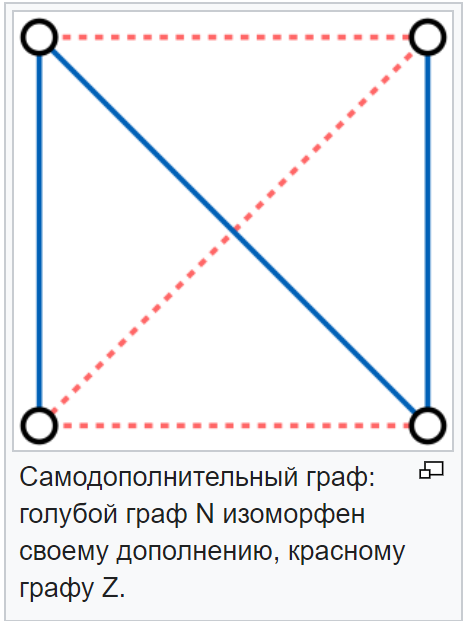
\includegraphics[scale = 0.8]{pictures/week 4/4.1.png}
\end{center}

\begin{center}
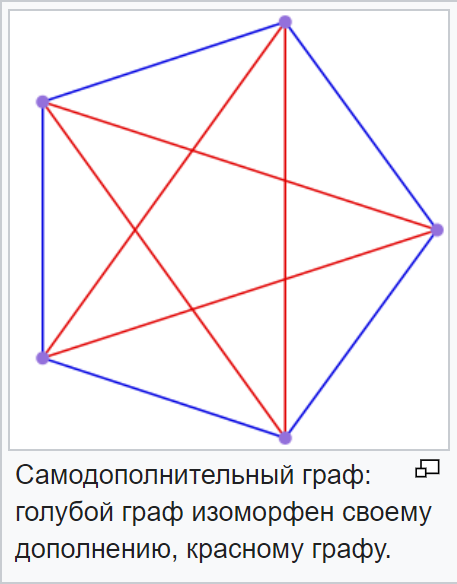
\includegraphics[scale = 0.8]{pictures/week 4/4.2.png}
\end{center}



\begin{flushright}
\begin{large}
\textbf {}
\end{large}
\end{flushright}

\section{Графы. Деревья и раскраски}

\subsection{Задача 1}


Степень каждой вершины графа равна 2. Верно ли, что этот граф
2-раскрашиваемый?
\begin{center}
\bfseries
{\Large Решение: }
\end{center}

По теореме "граф $G$ является двураскрашиваемым тогда и только тогда, когда в
нём нет циклов нечётной длины". Значит наличие у графа степеней всех вершин равных 2 не является достаточным условием, потому что может содержаться цикл нечётной длины. Пример наличия цикла нечетной длины -- граф-треугольник.

\begin{flushright}
\begin{large}
\textbf {нет }
\end{large}
\end{flushright}

\begin{center}
\subsection{Задача 2}
\end{center}

Докажите, что в дереве на $2n$ вершинах есть независимое множество
размера $n$ (ни одна пара вершин множества не соединена ребром). 
\begin{center}
\bfseries
{\Large Решение: }
\end{center}

Так как любое дерево 2-раскрашиваемо (существует правильная раскраска в 2 цвета), то количество вершин какого-то одного цвета будет не меньше, чем $n$, иначе получим, что $(x,y<n),$ а $ x+y < 2n$, а кол-во вершин должно равняться $2n$. То же самое по принципу Дирихле. Тогда возьмем $n$ вершин цвета, который встречается раз не меньше, чем $n$, все эти вершины будут раскрашены в один цвет и, соответственно, не будут смежными, тогда они будут составлять независимое множество размера $n$.

То, что любое дерево 2-раскрашиваемо (существует правильная раскраска в 2 цвета) легко можно доказать:

Вершина $v $ связана с каждой вершиной $u$ дерева $T$ единственным простым путем
$p_u$. Если длина $|p_u|$ пути $p_u$ четна, окрасим $u$ в белый цвет, иначе — в черный. Пусть
вершины $u$ и $w$ смежны. Если w не входит в путь $p_u$, то $p_w = p_uw$; в противном
случае $|p_w| < |p_u|$, а значит, $u$ не входит в $p_w$ и $p_u = p_wu$. В каждом из случае
числа $|p_u|$ и $|p_w|$ разной четности. Следовательно, вершины $ u$ и $w$ разного цвета и раскраска правильная.\\



\begin{flushright}
\begin{large}
\textbf {доказано}
\end{large}
\end{flushright}
\newpage

\begin{center}
\subsection{Задача 3}
\end{center}

 В дереве на $2020$ вершинах ровно три вершины имеют степень $1$.
Сколько вершин имеют степень $3$? 
\begin{center}
\bfseries
{\Large Решение: }
\end{center}

Очевидно, что вершины со степенью $degA \geqslant 4$ не может быть:

Если бы такая вершина существовала, то из такой вершины как минимум существовало бы 4 пути таких, что они заканчиваются на вершинах со степенью 1, иначе появился бы цикл. Значит было бы как минимум $degA$ вершин со степенью 1, что противоречит условиям. Значит $degA_{max} = 3$.

Так как из вершины $A$ в каждую вершину со степенью 1 ведет ровно 1 путь, то такая вершина обязательно должна существовать и она единственна.

\begin{flushright}
\begin{large}
\textbf {одна вершина со степенью 3 }
\end{large}
\end{flushright}


\begin{center}
\subsection{Задача 4}
\end{center}

Есть два дерева на $ n$ вершинах, каждое имеет диаметр длины $d$.
Можно ли так добавить ребро между вершинами этих деревьев, чтобы
длина диаметра полученного дерева равнялась $d$? 
\begin{center}
\bfseries
{\Large Решение: }
\end{center}

Стоит сразу понять, что диаметр будет не меньше, чем исходный диаметр $d$, так как новое ребро никаким образом не уменьшит максимальное из расстояний между двумя вершинами исходных деревьев.

По принципу Дирихле наименьший возможный диаметр $d^{\textbf{'}}$ будет, если разместить ребро между центрами деревьев, то есть между их вершинами $\frac{n}{2}$. Если ребро соединяет деревья в другиъ точках, то с каждым сдвигом от центра $d^{\textbf{'}}$ будем увеличиваться на 2. Теперь найдем минимально возможный $d^{\textbf{'}}$. Он будет равен $d^{\textbf{'}} = \frac{d}{2} + \frac{d}{2}+ 1$, (1 -- длина ребра). Отсюда получаем, что $d^{\textbf{'}} = d + 1 > d$. Итак, нельзя добавить ребро между двумя дереьвями с одинаковыми диаметрами так, чтобы диаметр нового дерева равнялся старым.

\begin{flushright}
\begin{large}
\textbf {нельзя }
\end{large}
\end{flushright}


\begin{center}
\subsection{Задача 5}
\end{center}

 Докажите, что если степень каждой вершины графа не превосходит
$d$, то его можно правильно раскрасить в $d + 1$ цвет.
\begin{center}
\bfseries
{\Large Решение: }
\end{center}

Будем раскрашивать вершины в различные цвета и в произвольном порядке.
На цвет каждой очередной вершины имеется не более $d$ запретов, поэтому
мы сможем ее окрасить в $d+1$ цвет.\\

\begin{flushright}
\begin{large}
\textbf {доказано}
\end{large}
\end{flushright}


\begin{center}
\subsection{Задача 6}
\end{center}

 Назовем не 2-раскрашиваемый граф минимальным, если после уда-
ления любого ребра он становится 2-раскрашиваемым. Докажите, что
в минимальном не 2-раскрашиваемом графе на 1000 вершинах есть
хотя бы одна изолированная вершина (т. е. вершина степени 0).
\begin{center}
\bfseries
{\Large Решение: }
\end{center}

По лемме граф не $2$-раскрашиваемый, если в нем содержиться цикл нечетной длины. Так как по условию минимально не 2-раскрашиваемого графа удаление любого ребра ведет к тому, что граф становиться 2-раскрашиваемым, а значит и исчезает цикл нечетной длины, получаем, что любое ребро -- это часть нечетного цикла, а значит и весь граф -- это нечетный цикл, значит в нём содержится нечётное количество вершин, максимальное количество вершин в графе, состоящих в цикле -- $999$, значит существует как минимум $1$ изолированная вершина.\\ 

\begin{flushright}
\begin{large}
\textbf {доказано }
\end{large}
\end{flushright}


\begin{center}
\subsection{Задача 7}
\end{center}

 Пусть $G$ — связный граф, который не является графом-путём и
$|V (G)| > 3$. Докажите, что в $G$ есть три вершины $v_1, v_2, v_3$, в результате
удаления которых вместе со всеми смежными рёбрами, получается
связный граф $G^{\textbf{'}} = G [V \setminus \{v_1,v_2,v_3 \} ]$.
\begin{center}
\bfseries
{\Large Решение: }
\end{center}

Рассмотрим любой связный граф. Легко показать, что у любого связного графа есть остовное дерево:


Докажем индукцией по числу ребер $n$ ($n \geqslant 0$).

База индукции $n = 0$. Очевидно, получаем множества не связных подграфов графа $G$ , состоящих просто из $1$ вершины. А так как одна вершина -- это дерево, то все выполняется.

Пусть при $n=k$ выполняется. Докажем для $n = k + 1$.

Если в графе $G$ есть ребро, после удаления которого граф $G$ остается связным и, получается, имеет кол-во ребер $|E| = n = k$,  что по предположению индукции верно, тогда имеем граф $G(|E| = k+1)$, который имеет остовое дерево и подходит для $G$.

Если такого ребра нет, то получаем после удаления несвязный граф и, соответсвенно, будет остовное дерево, так как несвязный граф состоит из изолированных вершин или связных графов, тогда остовное дерево есть по индукции или по определению в изолированной вершине.

В данном дереве есть хотя бы одна вершина степени 1 и мы можем удалить ее, а остальные вершины остануться связными, а следовательно и граф останется связным.

Таким образом в любом связном графе можно найти остовное дерево и такую вершину и, соответсвтенно мы можем проделать такую операцию $3$ раза (после каждого раза у нас будет связный граф), получим $G^{\textbf{'}} = G[V\setminus \{ v_1,v_2,v_3\} ]$.

\begin{flushright}
\begin{large}
\textbf {доказано }
\end{large}
\end{flushright}


\begin{center}
\subsection{Задача 8}
\end{center}

 Граф получен из графа-цикла $C_{2n}$, $n > 2$ добавлением рёбер, соеди-
няющих противоположные вершины ($v_1$ соединена с $v_{n+1}, v_2$ с $v_{n+2}$ и т.д.).При каких $n$ получившийся граф правильно раскрашиваемый

{\bf a)} в два цвета; {\bf б)} в три цвета?
\begin{center}
\bfseries
{\Large Решение: }
\end{center}

{\bf a)} Так как цикл чётной длины является 2-раскрашиваемым, тут же возникает необходимое условие: $V_1$ и $V_{n + 1}$ разного цвета, значит 1 и $n+1$ должны быть разной чётности $ \Rightarrow n$ должно быть нечётным.

{\bf б)} Так как при $n$ - нечётном можно раскрасить в $2$ цвета, то и в тоже $3$ можно. Рассмотрим $n$ - чётное.

Тогда можно раскрасить следующим образом : $A_{2k+1}$ -- в один цвет, где $2k+1 < n+1$; $A_{2m}$ -- в другой, где $m < n+1$, а элементы $A_{2n}$ и $A_{n+1}$ в третий цвет. Тогда у нас получится правильная окраска. Сразу стоит отметить ограничение на $k$, поэтому $n > 2$. 

\begin{flushright}
\begin{large}
\textbf {Ответ: {\bf a)} $n$ -- нечетное.\\
{\bf б)} любое $n > 2$.}
\end{large}
\end{flushright}


\begin{center}
\subsection{Задача 9}
\end{center}

 В графе на $100$ вершинах, каждая из которых имеет степень $3$, есть
ровно $600$ путей длины $3$. Сколько в этом графе циклов длины $3$?
\begin{center}
\bfseries
{\Large Решение: }
\end{center}

Так как путь не должен проходить по одному и тому же ребру $2$ раза, то такой путь имеет вид $E_1E_2E_3$. Осталось посчитать, сколькими способами мы можем выбрать эти ребра.

Сначала выбираем ребро $E_2$, оно определяется началом и концом. Начало -- любая вершина; способов выбрать -- $100$ . Конец -- любая из трёх соседних вершин. Итого $300$ способов выбрать $E_2 = \{ u ; v\}$.

Ребро $E_1$ можно выбрать $4$ способами: $2$ способа со стороны вершины $u$ и $2$ способа со стороны вершины $v$. Итого $1200$ способов выбора пути из трёх рёбер.

Так как по условию путей $600$, то остальные $600$ -- это построенные нашими рассуждениями циклы (больше вариантов построения графа на $3$ рёбрах нет). Но нужно учесть, что нам не важен порядок выбора вершин при построении цикла, то есть мы посчитали в $3!$ раз больше, чем реализуется на самом деле. Значит получаем $100$ различных циклов.


\begin{flushright}
\begin{large}
\textbf {Ответ: 100 циклов }
\end{large}
\end{flushright}


\begin{center}
\subsection{Задача 10}
\end{center}

 Докажите, что если размер максимальной клики в графе четный,
то можно раскрасить вершины графа в два цвета так, что размеры
максимальных клик в подграфах обоих цветов равны (подграф инду-
цирован множеством вершин одного цвета).
\begin{center}
\bfseries
{\Large Решение: }
\end{center}


Пусть у нас в общем случае имеется несколько клик максимального размера в графе. Заметим, что у нас не может быть такого, что объединение каких-то двух клик максимального размера в графе -- клика большего размера, так как мы уже рассматриваем максимальные по размеру клики.

Рассмотрим случай, когда у клик максимального размера $n$ в графе чётное количество вершин. Тогда раскрасим эти клики так, чтобы $\frac{n}{2}$ вершин были раскрашены в первый цвет, а остальные вершины -- во второй, тогда у нас в подграфах обоих цветов должны быть одинаковые размеры максимальных клик $\frac{n}{2}$. Для этого вершины остальных клик в графе до раскраски надо раскрасить следующим образом: если число вершин чётное, то раскрасим эти клики так же, как мы уже раскрасили клики максимальных размеров, а если число вершин нечётное и равно $2k + 1$, то $k$ вершин раскрашиваем в первый цвет и $k+1$ во второй. В этом случае получаем, что $k+1 \leqslant \frac{n}{2}$ и $k < \frac{n}{2}$ -- в любом случае получается клика по размеру, не превосходящему $\frac{n}{2}$. 

Все остальные вершины раскрашиваем произвольным образом, так как они не входят в клики и после раскраски тоже не будут входить в клики.

Заметим, что если в графе пересекаются клики максимальных размеров, то мы всё равно можем их раскрасить описанным выше способом: если рассмотреть только 1-ую клику, забыв, что она имеет общие вершины с другой, то в 1-ой клике после раскраски всегда получаем две клики в обоих подграфах размерами $\frac{n}{2}$ (описано выше), аналогично из 2-ой клики можно получить две клики в обоих подграфах размерами $\frac{n}{2}$.

Если же в графе и вовсе одна клика максимального размера, то тогда не возникает проблем с пересечением клик.

Если есть пересечение клик максимального и не максимального размеров, то применим описанные ранее рассуждения для пересечения двух клик максимального размера, за исключением того, что клика меньшего размера разбивается после раскраски на клики размеров $k+1 \leqslant \frac{n}{2}$ и $k < \frac{n}{2}$ или $k < \frac{n}{2}$ и $k < \frac{n}{2}$, где $2k+$ или $2k$ -- размеры клики меньшего размера. Тогда и в этом случае получаем две клики максимального размера в обоих подграфах.

\begin{flushright}
\begin{large}
\textbf {Доказано}
\end{large}
\end{flushright}



\end{document}
